%%%%%%%%%%%%%%%%%%%%%%%%%%%%%%%%%%%%%%%%%
% Beamer Presentation
% LaTeX Template
% Version 1.0 (10/11/12)
%
% This template has been downloaded from:
% http://www.LaTeXTemplates.com
%
% License:
% CC BY-NC-SA 3.0 (http://creativecommons.org/licenses/by-nc-sa/3.0/)
%
%%%%%%%%%%%%%%%%%%%%%%%%%%%%%%%%%%%%%%%%%

%----------------------------------------------------------------------------------------
%	PACKAGES AND THEMES
%----------------------------------------------------------------------------------------

\documentclass{beamer}

\mode<presentation> {

% The Beamer class comes with a number of default slide themes
% which change the colors and layouts of slides. Below this is a list
% of all the themes, uncomment each in turn to see what they look like.

%\usetheme{default}
%\usetheme{AnnArbor}
%\usetheme{Antibes}
%\usetheme{Bergen}
%\usetheme{Berkeley}
%\usetheme{Berlin}
%\usetheme{Boadilla}
%\usetheme{CambridgeUS}
%\usetheme{Copenhagen}
%\usetheme{Darmstadt}
%\usetheme{Dresden}
%\usetheme{Frankfurt}
%\usetheme{Goettingen}
%\usetheme{Hannover}
%\usetheme{Ilmenau}
%\usetheme{JuanLesPins}
%\usetheme{Luebeck}
%\usetheme{Madrid}
%\usetheme{Malmoe}
%\usetheme{Marburg}
%\usetheme{Montpellier}
%\usetheme{PaloAlto}
%\usetheme{Pittsburgh}
%\usetheme{Rochester}
%\usetheme{Singapore}
%\usetheme{Szeged}
\usetheme{Warsaw}

% As well as themes, the Beamer class has a number of color themes
% for any slide theme. Uncomment each of these in turn to see how it
% changes the colors of your current slide theme.

%\usecolortheme{albatross}
%\usecolortheme{beaver}
%\usecolortheme{beetle}
%\usecolortheme{crane}
%\usecolortheme{dolphin}
%\usecolortheme{dove}
%\usecolortheme{fly}
%\usecolortheme{lily}
%\usecolortheme{orchid}
%\usecolortheme{rose}
%\usecolortheme{seagull}
\usecolortheme{seahorse}
%\usecolortheme{whale}
%\usecolortheme{wolverine}

%\setbeamertemplate{footline} % To remove the footer line in all slides uncomment this line

%\setbeamertemplate{footline}[page number] % To replace the footer line in all slides with a simple slide count uncomment this line

%\setbeamertemplate{navigation symbols}{} % To remove the navigation symbols from the bottom of all slides uncomment this line
}

% insert page number in footer 
\addtobeamertemplate{navigation symbols}{}{%
    \usebeamerfont{footline}%
    \usebeamercolor[fg]{footline}%
    \hspace{1em}%
    \insertframenumber/\inserttotalframenumber
}

\usepackage{graphicx} % Allows including images
\usepackage{booktabs} % Allows the use of \toprule, \midrule and \bottomrule in tables
\usepackage{amsmath}
\usepackage{bbm} % Allows indicator variables 

\AtBeginSection[]
{
   \begin{frame}
       \frametitle{Outline}
       \tableofcontents[currentsection]
   \end{frame}
}

%----------------------------------------------------------------------------------------
%	TITLE PAGE
%----------------------------------------------------------------------------------------

\title[Intro to Concentration Inequalities]{A High-Level Introduction to Concentration Inequalities} % The short title appears at the bottom of every slide, the full title is only on the title page

\author{Haoen CUI} % Your name
\institute[Uptake] % Your institution as it will appear on the bottom of every slide, may be shorthand to save space
{
Uptake Math Club Lightning Talk
% Your institution for the title page
% Your email address
}
%\date{\today} % Date, can be changed to a custom date
\date{July 5, 2019}

\begin{document}

\begin{frame}
\titlepage % Print the title page as the first slide
\end{frame}

%----------------------------------------------------------------------------------------
%	PRESENTATION SLIDES
%----------------------------------------------------------------------------------------

%------------------------------------------------
\section{Introduction} 
%------------------------------------------------

\subsection{Objectives} 
\begin{frame}
\frametitle{Objectives} 

What are ``concentration inequalities'' used for? 
\begin{itemize}
    \item To show that some random quantity is close to its mean with high
probability
\end{itemize}

Why does it matter? 
\begin{itemize}
    \item To prove theoretical statistical learning results
\end{itemize}


\end{frame}

%------------------------------------------------

\subsection{Notation} 
\begin{frame}
\frametitle{Notation} 

Let $P$ be a probability measure over an instance space $\mathcal{Z}$ and $f$ be a function defined on domain $\mathcal{Z}$, then we write 
\begin{align*}
P(f)   &\stackrel{\text{def}}{=} \mathbb{E}_{Z \sim P}[f(Z)] \\ 
P_n(f) &\stackrel{\text{def}}{=} \frac{1}{n}\sum_{i=1}^{n} f(Z_i) = \mathbb{E}_{Z \sim P_n}[f(Z)]
\end{align*}
where $Z_i \stackrel{\text{iid}}{\sim} P$ are sample observations and hence $P_n$ is the empirical measure, 
$$ P_n(A) = \frac{1}{n} \sum_{i=1}^{n} \mathbbm{1}\{Z_i \in A\} $$

\end{frame}

%------------------------------------------------

\subsection{High-Level Overview} 
\begin{frame}
\frametitle{Desired Concentration Inequalities} 

In general, we seek for results of the form 
$$ \mathbb{P}\bigg( \big| f(Z_1, \dots, Z_n) - \mathbb{E}[f(Z_1, \dots, Z_n)] \big| > \epsilon \bigg) < \delta(\epsilon, n) $$
where $\forall \epsilon > 0$, $\delta(\epsilon, n) \rightarrow 0 $ as $n \rightarrow \infty$. 

For statistical learning theory, we will need \textit{uniform bounds} of the form
$$ \mathbb{P}\bigg( \sup_{f \in \mathcal{F}} \big| f(Z_1, \dots, Z_n) - \mathbb{E}[f(Z_1, \dots, Z_n)] \big| > \epsilon \bigg) < \delta(\epsilon, n) $$
over a class of functions $\mathcal{F}$. 

\end{frame}

%------------------------------------------------

\begin{frame}
\frametitle{Application: Empirical Risk Minimization in Classification} 

Consider a binary classification problem. Suppose we have data $\{(X_i, Y_i)\}_{i=1}^{n}$ where $X_i \in \mathbb{R}^d$ and $Y_i \in \{0,1\}$. Let $f: \mathbb{R}^d \rightarrow \{0,1\}$ be a classifier, then its 
\begin{itemize}
    \item Training Error $$ \widehat{R}_{n}(f) \stackrel{\text{def}}{=} \frac{1}{n}\sum_{i=1}^{n} \mathbbm{1}\{ Y_i \neq f(X_i) \} $$ 
    \item Generalization Error: $$ R(f) = \mathbb{P}(Y \neq f(X)) $$
\end{itemize}

\end{frame}

%------------------------------------------------

\begin{frame}
\frametitle{Application: ERM in Classification (Cont.)} 

Let $\widehat{f}_{*}$ minimize training error $\widehat{R}_{n}$ and $f_{*}$ minimize generalization error $R$. Suppose we have 
$$ \sup_{f \in \mathcal{F}} | \widehat{R}_{n}(f) - R(f) | \leq \epsilon $$
then
$$ R(f_{*}) \leq R(\widehat{f}_{*}) \leq \widehat{R}_{n}(\widehat{f}_{*}) + \epsilon \leq \widehat{R}_{n}(f_{*}) + \epsilon \leq R(f_{*}) + 2\epsilon $$
which translates to 
$$ | R(\widehat{f}_{*}) - R(f_{*}) | \leq 2\epsilon $$
guarantees the consistency of ERM over $\mathcal{F}$. 

\end{frame}

%------------------------------------------------
\section{Basic Inequalities} 
%------------------------------------------------

\subsection{Commonly Used Results} 
\begin{frame}
\frametitle{Commonly Used Results} 

\begin{block}{Tail Probability of Gaussian Random Variable Decays Exponentially}
For $\forall \epsilon > 0$, consider sample average $\overline{X}_n$, 
$$ X_i \stackrel{\text{iid}}{\sim} \mathcal{N}(\mu, \sigma^2) \implies \mathbb{P}(|\overline{X}_n - \mu| > \epsilon) \leq \exp \bigg( -\frac{n\epsilon^2}{2\sigma^2} \bigg) $$
\end{block}

\end{frame}

%------------------------------------------------

\begin{frame}
\frametitle{Commonly Used Results (Cont.)} 

\begin{block}{Bounds on Expected Values}
Suppose that $\mathbb{P}(X_n \geq 0) = 1$ and $\exists c_1 > \frac{1}{e}, c_2 >0$ such that $\forall \epsilon >0$
$$ \mathbb{P}(X_n < \epsilon) \leq c_1 \exp(-c_2 n \epsilon^2) $$
then we have, for $C = \frac{1 + \ln(c_1)}{c_2}$, 
$$ \mathbb{E}[X_n] \leq \sqrt{\frac{C}{n}} $$
\end{block}

\end{frame}

%------------------------------------------------

\begin{frame}
\frametitle{Commonly Used Results (Cont.)} 

\begin{block}{Bounds on the Maximum of a Set of Random Variables}
Let $\{X_i\}_i$ be a set of random variables. Suppose $\exists \sigma > 0$ such that 
$$ \mathbb{E}[ \exp(tX_i) ] \leq \exp\big( \frac{t\sigma^2}{2} \big) \qquad \forall t>0 $$
then 
$$ \mathbb{E} \bigg[ \max_{i \in [n]} X_i \bigg] \leq \sigma \sqrt{2 \ln(n)} $$
\end{block}

\end{frame}

%------------------------------------------------

\begin{frame}
\frametitle{Commonly Used Results (Cont.)} 

\begin{block}{Bounds on Moment Generating Functions}
Suppose $\mathbb{P}(|X| \leq c) = 1$ and $\mathbb{E}[X] = 0$. Let $ \sigma^2 \stackrel{\text{def}}{=} \text{Var}[X] $. Then $$ \mathbb{E}[e^{tX}] \leq \exp \bigg\{ t^2 \sigma^2 \bigg( \frac{e^{tc} - 1 - tc}{(tc)^2} \bigg) \bigg\} \qquad \forall t > 0 $$
\end{block}

\begin{block}{Another Bound on Moment Generating Functions Useful for Proof of Hoeffding's Inequality}
Suppose $\mathbb{P}(a \leq X \leq b) = 1$ and let $\mu \stackrel{\text{def}}{=} \mathbb{E}[X]$, then 
$$ \mathbb{E}[e^{tX}] \leq \exp \bigg( t\mu + \frac{(b-a)^2}{8} t^2 \bigg) \qquad \forall t \in \mathbb{R}$$
\end{block}

\end{frame}

%------------------------------------------------

\subsection{Commonly Used Concentration Inequalities} 
\begin{frame}
\frametitle{Roadmap} 

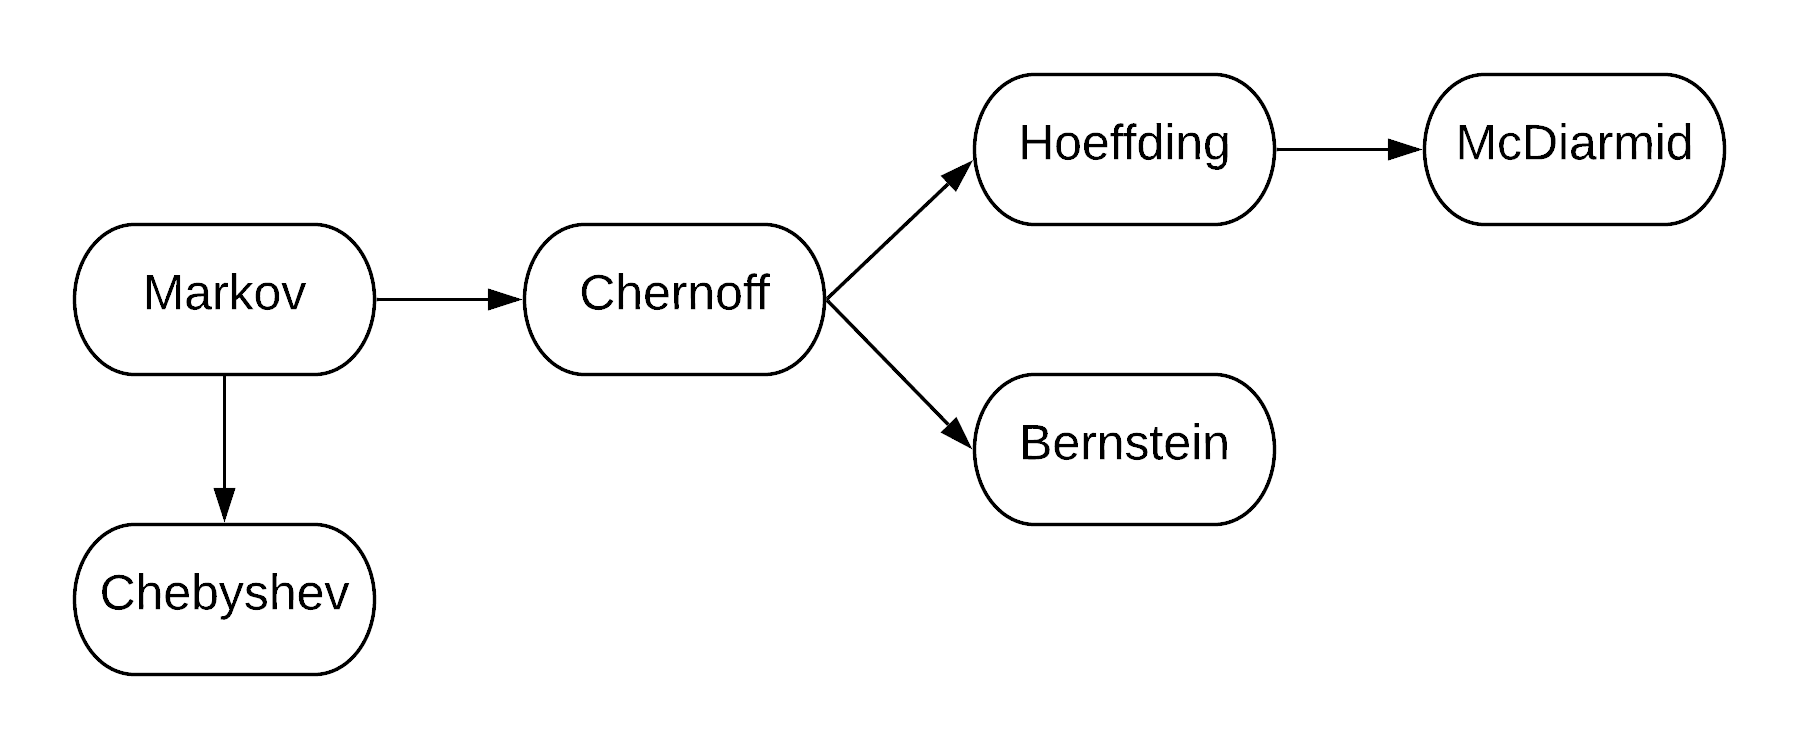
\includegraphics[width=\textwidth]{roadmap.png}

\end{frame}

%------------------------------------------------

\begin{frame}
\frametitle{Markov's Inequality and Chebyshev's Inequality} 

\begin{block}{Markov's Inequality}
Suppose that $\mathbb{P}(X \geq 0) = 1$ and $\mathbb{E}[X] < \infty $, then for $\forall \epsilon > 0$, 
$$ \mathbb{P}(X > \epsilon) \leq \frac{E[X]}{\epsilon} $$
\end{block}

\begin{block}{Chebyshev's Inequality (Corollary of Markov's Inequality)}
Suppose that $\mathbb{E}[X] < \infty $ and $\mathbb{E}[X^2] < \infty $, then for $\forall \epsilon > 0$, 
$$ \mathbb{P}(|X - \mathbb{E}[X]| > \epsilon) \leq \frac{\text{Var}[X]}{\epsilon^2} $$
\end{block}

\end{frame}

%------------------------------------------------

\begin{frame}
\frametitle{Chernoff Bounding Trick} 

Consider applying \textit{Chebyshev's Inequality} to sample average $\overline{X}_n$ of iid random variables with mean $\mu$ and variance $\sigma^2$, 
$$ \mathbb{P}(|\overline{X}_n - \mu| > \epsilon) \leq \frac{\sigma^2}{n\epsilon^2} $$
does not decay exponentially fast as sample size $n$ increases. 

\begin{block}{Chernoff Bounding Trick}
$$ \mathbb{P}(X > \epsilon) \leq \inf_{t \geq 0} e^{-t\epsilon}\mathbb{E}[e^{tX}] \qquad \forall \epsilon \in \mathbb{R} $$
\end{block}

\end{frame}

%------------------------------------------------

\begin{frame}
\frametitle{Hoeffding's Inequality} 

\begin{block}{Hoeffding's Inequality}
If $X_1, X_2, \cdots, X_n$ are independent (but not necessarily identical) random variables with 
$$ \mathbb{P}(a_i \leq X_i \leq b_i) = 1 $$
and common mean $\mathbb{E}[X_i] = \mu$, then for $\forall \epsilon > 0$ 
$$ \mathbb{P}(|\overline{X}_n - \mu| > \epsilon) \leq 2 \exp \bigg( -\frac{2n^2\epsilon^2}{\sum_{i=1}^{n} (b_i - a_i)^2} \bigg) $$
\end{block}

\end{frame}

%------------------------------------------------

\begin{frame}
\frametitle{McDiarmid's Inequality} 

McDiarmid's Inequality relaxes bounded random variable assumption in \textit{Hoeffding's Inequality} to \textit{bounded difference}. 
\begin{block}{McDiarmid's Inequality}
If $X_1, X_2, \cdots, X_n$ are independent random variables with 
$$ \sup_{z_1, \cdots, z_n, {z_i}'} \bigg\lvert f(\cdots, z_{i-1}, z_i, z_{i+1}, \cdots) - f(\cdots, z_{i-1}, {z_i}', z_{i+1}, \cdots) \bigg\rvert \leq c_i $$
for some constant vector $(c_1, \cdots, c_n)$, then 
$$ \mathbb{P}(|P_n(f) - P(f)| > \epsilon) \leq 2 \exp \bigg( -\frac{2\epsilon^2}{\sum_{i=1}^{n} {c_i}^2} \bigg) \qquad \forall \epsilon > 0 $$
\end{block}

\end{frame}

%------------------------------------------------

\begin{frame}
\frametitle{Bernstein's Inequality} 

\textit{Hoeffding’s inequality} does not use any information about the random variables except the fact that they are bounded. If the variance of $X_i$ is small, then we can get a sharper inequality from \textit{Bernstein’s inequality}.
\begin{block}{Bernstein’s Inequality}
Suppose $\mathbb{P}(|X_i| \leq c) = 1$ and $\mathbb{E}[X_i] = \mu$, then 
$$ \mathbb{P}(|\overline{X}_n - \mu| > \epsilon) \leq 2 \exp \bigg\{ - \frac{n\epsilon^2}{2\sigma^2 + \frac{2}{3}c\epsilon} \bigg\} \qquad \forall \epsilon > 0 $$
where $\sigma^2 \stackrel{\text{def}}{=} \frac{1}{n}\sum_{i=1}^{n} \text{Var}[X_i]$. 
\end{block}

\end{frame}

%------------------------------------------------
\section{Uniform Bounds} 
%------------------------------------------------

\subsection{Vapnik-Chervonenkis (VC) Dimension} 
\begin{frame}
\frametitle{Shattering Number} 

Let $\mathcal{F}$ be a class of binary functions $f: \mathcal{Z} \rightarrow \{0,1\}$ over instance space $\mathcal{Z}$. For any finite set $S = \{z_1, z_2, \cdots, z_n\} \subset \mathcal{Z}$, define \textit{projection of} $\mathcal{F}$ \textit{onto} $S$ as 
$$ \mathcal{F}_{S} \stackrel{\text{def}}{=} \bigg\{ \big( f(z_1), \cdots, f(z_n) \big): f \in \mathcal{F} \bigg\}  $$
Note that $\mathcal{F}_{S}$ is a finite collection of binary vectors and $|\mathcal{F}_{S}| < 2^n$. 

\begin{block}{Shattering Number}
$$ s(\mathcal{F}, n) \stackrel{\text{def}}{=} \sup_{z_1, z_2, \cdots, z_n \in \mathcal{Z}} |\mathcal{F}_{z_1, z_2, \cdots, z_n}| $$
\end{block}

\end{frame}

%------------------------------------------------ 

\begin{frame}
\frametitle{Shattering Number (Cont.)} 

\begin{block}{Example}
Consider instance space $\mathcal{Z} = \mathbb{R}$ and function class be positive rays $\mathcal{F} = \{\mathbbm{1}\{z > t\}: \mathcal{Z} \mapsto \{0,1\} | t \in \mathbb{R} \}$. Pick three real numbers $z_1 < z_2 < z_3$ and let $S = \{z_1, z_2, z_3\}$. Then 
$$ \mathcal{F}_{S} = \{ (0, 0, 0), (0, 0, 1), (0, 1, 1), (1, 1, 1) \} $$
\end{block}

\end{frame}

%------------------------------------------------ 

\begin{frame}
\frametitle{Vapnik-Chervonenkis (VC) Dimension} 

\begin{block}{Vapnik-Chervonenkis (VC) Dimension}
The \textit{Vapnik-Chervonenkis (VC) Dimension} of a class of binary function $\mathcal{F}$ is defined as 
$$ d_{\text{VC}}(\mathcal{F}) \stackrel{\text{def}}{=} \sup \big\{ n \in \mathbb{N}: s(\mathcal{F}, n) = 2^n \big\} $$
\end{block}

VC dimension can be think of as 
\begin{itemize}
    \item binary degrees of freedom, or 
    \item estimate of effective number of parameters. 
\end{itemize}

\end{frame}

%------------------------------------------------ 

\begin{frame}
\frametitle{VC Dimension: Collection of Results} 

\begin{table}[]
\begin{tabular}{@{}ll@{}}
\toprule
\multicolumn{1}{c}{Binary Function Class $\mathcal{F}$} & \multicolumn{1}{c}{$d_{\text{VC}}(\mathcal{F})$} \\ \midrule
Finite set with $N$ elements & $\log_2(N)$ \\
Intervals $[a,b] \subset \mathbb{R}$ & 2 \\
Discs in $\mathbb{R}^2$ & 3 \\
Closed balls in $\mathbb{R}^d$ & $d+2$ \\
Rectangles in $\mathbb{R}^d$ & $2d$ \\
Half-spaces in $\mathbb{R}^d$ & $d+1$ \\
Convex polygons in $\mathbb{R}^d$ & $\infty$ \\ \bottomrule
\end{tabular}
\end{table}

\end{frame}

%------------------------------------------------ 

\begin{frame}
\frametitle{VC Dimension: Example} 

VC dimension works like this: 
\begin{itemize}
    \item You choose the points, 
    \item then the adversary chooses the labeling such that 
    \item there always exists a function $f$ that can correctly classify the specified labeling of those points.
\end{itemize}
If you are able to succeed for all labelings of the adversary, we say that the VC dimension of binary function class $\mathcal{F}$ is at least the number of points you were able to choose.
\begin{block}{VC Dimension of Intervals $[a, b]$ on $\mathbb{R}$ is 2}
\begin{itemize}
    \item Any two-point set can be shattered  
    \item No three-point set can be shattered (Consider $\{(a, 1), (b, 0), (c, 1)\}$ with $a < b < c$)
\end{itemize}
\end{block}

\end{frame}

%------------------------------------------------ 

\begin{frame}
\frametitle{Finite VC Dimensional Function Classes Has Bounded Shattering Number} 

If the VC dimension is finite, then the growth function cannot grow too quickly. In
fact, there is a phase transition: 
\begin{itemize}
    \item for $n < d$, $s(\mathcal{F}, n) = 2^n$, and  
    \item then the growth switches to polynomial $s(\mathcal{F}, n) \sim \mathcal{O}(n^d)$
\end{itemize}
\begin{block}{Sauer-Shelah Lemma}
Suppose $d_{\text{VC}}(\mathcal{F}) = d$, then 
$$ s(\mathcal{F}, n) \leq \sum_{i=0}^{d} \binom{n}{i} $$ 
In particular, when $n \geq d$, 
$ s(\mathcal{F}, n) \leq \big( \frac{en}{d} \big)^d $. 
\end{block}

\end{frame}

%------------------------------------------------ 

\begin{frame}
\frametitle{Application: Bound Generalization Error} 

For a binary function class $\mathcal{F}$ that is not too complex, consistency of generalization is guaranteed. One can think of it as a bias-variance trade-off: 
\begin{itemize}
    \item Bias: training error $P_n(f)$
    \item Variance: ``confidence internal'' on the right-hand side of the inequality 
\end{itemize}

\begin{block}{}
Suppose $d_{\text{VC}}(\mathcal{F}) < \infty$, then with probability at least $1 - \delta$, 
$$ \sup_{f \in \mathcal{F}} | P_n(f) - P(f) | \leq \sqrt{\frac{8}{n}\bigg( \ln\big( \frac{4}{\delta} \big) + d_{\text{VC}}(\mathcal{F}) \big( 1 + \ln\big( \frac{n}{d_{\text{VC}}(\mathcal{F})} \big) \big) \bigg)} $$
\end{block}

\end{frame}

%------------------------------------------------ 

\subsection{Rademacher Complexity} 
\begin{frame}
\frametitle{Rademacher Complexity} 

\begin{block}{Rademacher Complexity of $\mathcal{F}$}
Consider \textit{Rademacher random variables} $\sigma_i \stackrel{\text{iid}}{\sim} \text{Uniform}(\{-1, 1\})$, define 
$$ \text{Rad}_n(\mathcal{F}) \stackrel{\text{def}}{=} \mathbb{E}_{Z}\bigg[ \mathbb{E}_{\sigma}\bigg[ \sup_{f \in \mathcal{F}} \bigg| \frac{1}{n}\sum_{i=1}^{n} \sigma_i f(Z_i) \bigg| \bigg] \bigg] $$
\end{block}
Rademacher complexity generalizes correlation. Notice that 
$$ \widehat{R}_{n}(f) \stackrel{\text{def}}{=} \frac{1}{n}\sum_{i=1}^{n} \mathbbm{1}\{ Y_i \neq f(X_i) \} = \frac{1}{2} - \frac{1}{2n}\sum_{i=1}^{n} Y_if(X_i)$$
This gives us Rademacher correlation: what's the best that an algorithm can do on random labels. 

\end{frame}

%------------------------------------------------ 

\begin{frame}
\frametitle{Rademacher Complexity Extends Shattering Number and VC Dimension} 

\textit{Rademacher Complexity} is defined on a class of bounded functions. 
\begin{block}{In the special case where $\mathcal{F}$ is a class of binary functions,}
$$ \text{Rad}_n(\mathcal{F}) \leq \sqrt{\frac{2}{n} \ln\big( s(\mathcal{F}, n) \big)} \qquad \forall n \in \mathbb{N} $$
\end{block}

\begin{block}{Devroye and Lugosi (2001)}
Suppose $d_{\text{VC}}(\mathcal{F}) < \infty$, then $\exists$ universal constant $C > 0$, 
$$ \text{Rad}_n(\mathcal{F}) \leq C \sqrt{\frac{d_{\text{VC}}(\mathcal{F})}{n}} $$
\end{block}

\end{frame}

%------------------------------------------------ 

\begin{frame}
\frametitle{Application: Bound Generalization Error} 

\begin{block}{}
With probability at least $1 - \delta$, 
$$ \sup_{f \in \mathcal{F}} | P_n(f) - P(f) | \leq 2 \text{Rad}_n(\mathcal{F}) + \sqrt{\frac{1}{2n} \ln \bigg( \frac{2}{\delta} \bigg)} $$
\end{block}

Combining everything together, we have showed a generalization error bound for any learning algorithm $\mathcal{F}$ using ERM 
\begin{block}{}
With probability at least $1 - \delta$, 
$$ R(\widehat{f}_{*}) \leq R(f_{*}) + 4 C \sqrt{\frac{d_{\text{VC}}(\mathcal{F})}{n}} + \sqrt{\frac{2}{n} \ln \bigg( \frac{2}{\delta} \bigg)} $$
\end{block}

Concentration of measure is a vast and still growing area. Literature contains many refinements and extensions of these results. 

\end{frame}

%------------------------------------------------

\section*{}
\begin{frame}
\Huge{\centerline{Questions?}}
\end{frame}

%----------------------------------------------------------------------------------------

\end{document}